\documentclass[aps,letterpaper,11pt]{revtex4}


\usepackage{graphicx} % For images
\usepackage{float}    % For tables and other floats
\usepackage{verbatim} % For comments and other
\usepackage{amssymb}  % For more math
\usepackage{fullpage} % Set margins and place page numbers at bottom center
\usepackage{listings} % For source code
\usepackage[usenames,dvipsnames]{color} % For colors and names
\usepackage[pdftex]{hyperref}           % For hyperlinks and indexing the PDF
\usepackage{pdfpages}
\usepackage{subfigure}

\usepackage{listings}
\usepackage[usenames,dvipsnames,svgnames,table]{xcolor}
\usepackage{color}
\usepackage{textcomp}
\usepackage[utf8]{inputenc}

% Default fixed font does not support bold face
\DeclareFixedFont{\ttb}{T1}{txtt}{bx}{n}{12} % for bold
\DeclareFixedFont{\ttm}{T1}{txtt}{m}{n}{12}  % for normal

% Custom colors
\definecolor{deepblue}{rgb}{0,0,0.5}
\definecolor{deepred}{rgb}{0.6,0,0}
\definecolor{deepgreen}{rgb}{0,0.5,0}

% Python style for highlighting
\newcommand\pythonstyle{\lstset{
language=Python,
basicstyle=\ttm,
otherkeywords={self},             % Add keywords here
keywordstyle=\ttb\color{deepblue},
emph={MyClass,__init__},          % Custom highlighting
emphstyle=\ttb\color{deepred},    % Custom highlighting style
stringstyle=\color{deepgreen},
frame=tb,                         % Any extra options here
showstringspaces=false            % 
}}

\newcommand\launchstyle{\lstset{
    language=xml,
    tabsize=3,
    %frame=lines,
    frame=tb,
    rulesepcolor=\color{gray},
    xleftmargin=20pt,
    framexleftmargin=15pt,
    otherkeywords={node,include,param},
    keywordstyle=\ttb\color{deepblue},
    commentstyle=\color{orange},
    stringstyle=\color{deepgreen},
    breaklines=true,
    showstringspaces=false,
    basicstyle=\ttm,
    emph={pkg,args,value,file,name,type},
    emphstyle={\color{deepred}}}
    }


% Python environment
\lstnewenvironment{python}[1][]
{
\pythonstyle
\lstset{#1}
}
{}


% Launch for external files
\newcommand\pythonexternal[2][]{{
\launchstyle
\lstinputlisting[#1]{#2}}}

% Python for external files
\newcommand\launchexternal[2][]{{
\pythonstyle
\lstinputlisting[#1]{#2}}}

% Python for inline
\newcommand\pythoninline[1]{{\pythonstyle\lstinline!#1!}}
 
\hypersetup{ % play with the different link colors here
    colorlinks,
    citecolor=black,
    filecolor=black,
    linkcolor=black,
    urlcolor=black % set to black to prevent printing blue links
}

\newcommand{\labno}{Technical report}
\newcommand{\labtitle}{Motion Control on TurtleBot}
\newcommand{\authorname}{Kevin Descharrieres, Antoine Merlet}
\newcommand{\professor}{Dr. Ralph Seulin}






\begin{document}  
\begin{titlepage}
\begin{center}
{\LARGE \textsc{\labno:} \\ \vspace{4pt}}
{\Large \textsc{\labtitle} \\ \vspace{4pt}} 
\rule[13pt]{\textwidth}{1pt} \\ \vspace{150pt}
{\large By: \authorname \\ \vspace{10pt}
Professor: \professor \\ \vspace{10pt}
\today}
\end{center}




\end{titlepage}% END TITLE PAGE %%%%%%%%%%%%%%%%%%%%%%%%%%%%%%%%%%
\newpage
\tableofcontents
\newpage
\section{BRAINSTORM}
video
pict
command line
python
screenshots: consols -> what is started on which computer(ssh)
			 rviz : Part1 Goal 4, Part 2, Part 3

PART 1

BACK AND FORTH
mostly from ROS by example Vol. 1
Here we can see that the robot does not end at the starting position. In fact, the twist topic is not sufficient by itself to properly drive the robot, as is just emit Linear and Angular velocities and does not give any feedback. We need to add more sensing to make it viable
BACK AND FORTH WITH ODOMERTY
Odometry is our savior. It allows us to get information on the internal motion of the robot, and therefore check if the Twist messages are well applied. 

\newpage

%%%%%%% THE WRITING STARTS HERE %%%%%%
\section{Presentation of the robot}

\begin{figure}[H]\launchstyle
	\centering
	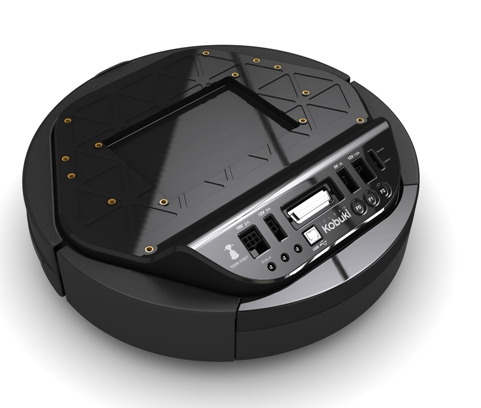
\includegraphics[height=8cm]{Mobile-Robot-Kobuki.jpg}
	\caption{Kobuki Base}
	\label{fig:Robot Base}    
\end{figure}

The first version of the TurtleBot was created in 2011 by Willow Garage society. This robot hardware, based on a vacuum cleaner, has been improved over the time and is now considered as a pillar of the robotic field. The aim of this robot is to make it affordable for a beginner in the field while being powerful enough for high-end applications. Moreover, the TurtleBot OS is based on the middle-ware ROS (Robot Operating System), making it a really nice tool as ROS is becoming more and more popular. By now, the TurtleBot became THE reference in education and research.

As any first version of a hardware/software, the TurtleBot could be improved, giving therefore the TurtleBot 2 (the one we are equipped with). Following are presented the main features of this robot:

\begin{itemize}
\item {A comfortable operating time (2-3 hours);}
\item {A Kinect for 3D sensing;}
\item {A fast charging Dock for idling charge;}
\item {A charging cable in order to charge the base while using it;}
\item {Cliff and drop sensors;}
\item {A laptop;}
\item {And 3 collision sensors.}
\end{itemize}

\begin{figure}[H]
	\centering
	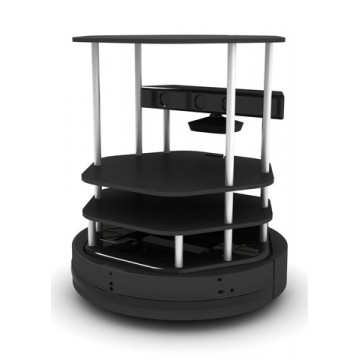
\includegraphics[height=8cm]{turtlebot-2-robot-mobile-ros.jpg}
	\caption{TurtleBot 2}
	\label{fig:Robot Components}    
\end{figure}

For more technical details about the Kobuki base, please refer to [1] (link it to the doc). Most all the work has been done using a very complete book: ROS by example, volume 1, R. Patrick Goebel.


\section{How to control a TurtleBot}
\subsection{Workspace and network}
There are mainly two ways of controlling the TurtleBot. 
The first option is to directly control the TurtleBot using the laptop connected to it. However, this is inconvenient as the TurtleBot might be moving, but also because the user does not have any comfortable position to use the laptop.

The second option is to remotely connect to the TurtleBot computer. This can be easily done with Ubuntu by using the SSH build-in command. Also, please notice that the network is already optimized in our case (singleton of the couple Workspace+TurtleBot per router), making the SSH really easy on our side. Therefore, you can distinguish two main components: the TurtleBot+laptop and the Workstation. This allows the control of the TurtleBot in an efficient (and comfortable) way. The only thing that is to be done to enable the remote control is to modify the bashrc file of the workstation (located in the Home folder in most of the cases, can be edited by using the command \textit{\$ gedit {\raise.17ex\hbox{$\scriptstyle\sim$}} /.bashrc}. The three last lines ('export') need to be uncommented. The first one should contain the IP address of the TurtleBot on your local network (most-likely starting by 192.168.XXX.XXX). The two second line should be filled with the IP of your Workstation. In order to make it easy for daily connection, we suggest that both the Workstation and the TurtleBot laptop are provided static IP addresses. 

In all the following, we will specify one which one should be started each command line. If not specified, the main computer (the workstation) should be considered as the default one.

\subsection{Topics and nodes}

A node represent a process, doing calculations. With ROS, each node is dedicated to a specific take. For example, one node manages the lidar, another on the Kinect, one the movement of the wheels, and so on. In order to communicate, Nodes are using Topics, by publishing messages into it. This topic has a specific name representing the type of data that it is carrying (the topic "joy" carries information about the joystick input). Node are not only publishing to topics, they can also subscribe to them, so that when a new topic publishes, they receive this data. This concepts are simple as long as the application is basic, otherwise, it is really complicated to figure out which node is publishing to which topic. In order to have a price idea of what is going on at a low level, a very powerful tool can be used: the rqt\_graph (presented later).

\subsection{Package}

A way to control the TurtleBot is to create a package. This allows to store several behaviours for the TurtleBot. In order to create such a package, one could either use the command 
\textit{\$ catkin\_create\_pkg \textless package \_name\textgreater [depend1] [depend2] [depend3]} by replacing the given parameters by the wanted name and dependencies. It is also possible to create manually a package from scratch, mostly for advanced users with a wide knowledge of ROS. In our case, we used the command \textit{\$ catkin\_create\_pkg project rospy std\_msgs}. Therefore, the package is named 'project' and is using two external libraries. Rospy is used to be able to create and run python scripts with the TurtleBot, and std\_msgs allowing to use standard data-types. The package also comes with a file named 'CMakeLists.txt', which we are not changing. The package also comes along with folders, such a scripts and launch files. For more documentation about packages, please follow \href{ http://wiki.ros.org/Packages}{this link}.

\subsection{Script}

In order to create your own routines for the robot, Scripts are used. They are mainly written in Python or C++ language, which are widely used in IT science, making it somewhat easy to create. Following is presented the basic commands to create a Python script for ROS.


\begin{python}
# Always import rospy for the script to work
import rospy

# Initializing a Self-created node called MyNode
rospy.init_node('MyNode')

# Declaring a new publisher to the Topic /cmd_vel. 
self.cmd_vel = rospy.Publisher('/cmd_vel', Twist, queue_size=1)
	
# Initialize the movement command that will be emitted to the publisher
move_cmd = Twist()

# Publishing the move_cmd message to the publisher (being /cmd_vel)
self.cmd_vel.publish(move_cmd)

# Putting the robot in sleep mode (usually when the script is done)
rospy.sleep(1)
\end{python}

Once the TurtleBot is started with a ROScore, it is possible to start scripts. However, having to start the ROScore with all the scripts needed for the experiment can be a bit tedious. Launch files can overcome this problem.

\subsection{Launch files}
Script file are simple to use, but not very convenient. Launch files bring the possibility to start several scripts and launch file as well as allowing to use custom settings. The following example show all of this.
\pythonexternal{class_joy2twist.launch}
As we can see on the first few lines, this launch file is starting another launch file. This included file may or may not include again other launch files, et caetera. From this, we can obviously see a big source of problem: any time you there is a need to debug one application, all launch files must be examined recursively. It is not unusual to have around seven layers of launch file.
In the launch files, it is also possible to set the values of parameters from the included nodes. Finally, it is also possible to remap some topics, transferring the published data to another topic. For more documentation about launch files, please follow \href{ http://wiki.ros.org/roslaunch/XML}{this link}.

\subsection{Bag files}
ROS is equipped with a very powerful tool to record all the topics and nodes while the robot is processing them: the bag files. It allows the user to save the robot state during an experiment so that it can be simulated later, or even re-run on the robot. We consider this tool really important, that is why we chose to provide a bag file corresponding to each script that we produced. To record a bag file with all the running topics, one can use the console command \textit{\$ rosbag record -a}. For more documentation about the rosbag command, please follow \href{http://wiki.ros.org/rosbag/Commandline}{this link}.

\section{Our project}
\subsection{Purpose}

\subsection{Simple motions, Twist and Odometry}
\subsection{Adding and controlling sensors}
\subsection{SLAM and ACML}
\section{Merging TurtleBot and PhantomX Arm Pincher}

\section{Challenges encountered}
\subsection{Hardware malfunctions}
	battery, desync, kinect, arm, arduino board
\subsection{Python}
	unknown libraries
\subsection{Debugging the TurtleBot}

\section{Conclusion}

\section{References}

\section{Appendix}



\section{OLD STUFF}
%Pictures of the different moves (subject)\launchstyle
The first move is the come-and-back which is a low level programming.
\begin{figure}[H]
	\centering
	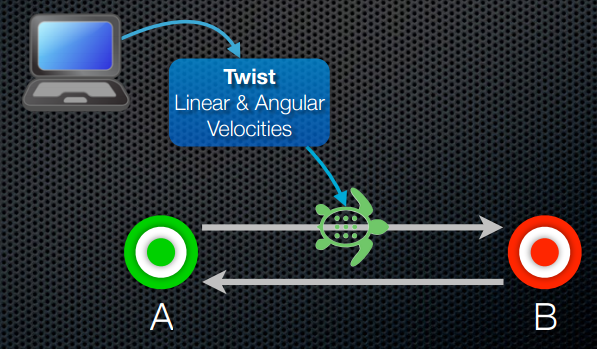
\includegraphics[height=8cm]{come-and-back.png}
	\caption{Come and Back movement}
	\label{fig: Come and Back movement}    
\end{figure}

The second one is the same movement as previously using the odometry data.
\begin{figure}[H]
	\centering
	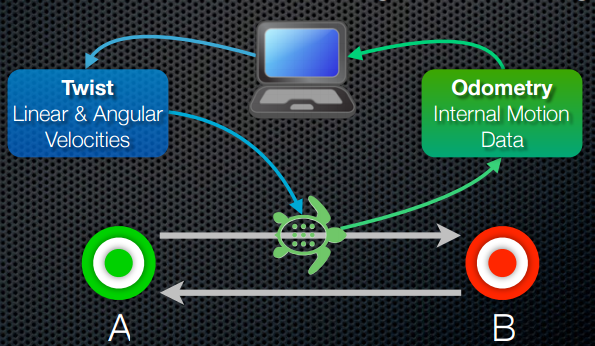
\includegraphics[height=8cm]{come-and-back-switch.png}
	\caption{Come and Back movement using odometry}
	\label{fig: Come and Back movement using odometry}    
\end{figure}


The third movement is navigating a square using twist and odometry.
\begin{figure}[H]
	\centering
	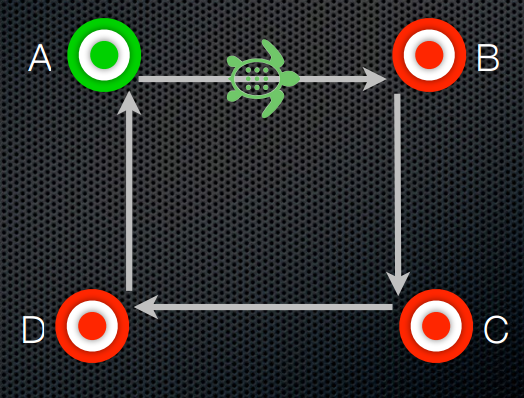
\includegraphics[height=8cm]{square.png}
	\caption{Square Movement}
	\label{fig: Square Movement}    
\end{figure}


The forth one is to follow a curve between a starting point and a target and navigation with path planing.
\begin{figure}[H]
	\centering
	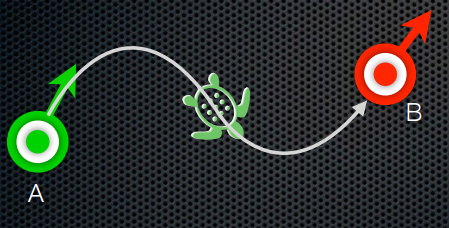
\includegraphics[height=8cm]{curve.png}
	\caption{Curve Movement}
	\label{fig: Curve Movement}    
\end{figure}



\section{Challenges}
\subsection{Twist}

The first main problem in this exercise was how to twist the TurtleBot in real time. For that, we had in a first time try to give it a rotation angle, for example 90 degrees, which is an angle easily recognizable. We saw quickly the problem, the describe angle was never 90 degrees, it was between 80 and 105 degrees. During the come-and-back demonstration, the move was great except the exact angle during the twist. This exercise demonstrated the fact that program a robot by giving it movement angle is not a good way if we want a precise result at the angle. Furthermore, it is useless to try to correct the angle by hand in the program because the describe angle will not be tow times the same, it changed at every step.

\subsection{Odometry}

\subsection{Basic Moves}

\section{ROSification}

\subsection{}

\subsection{}

\end{document} % DONE WITH DOCUMENT!


%https://www.generationrobots.com/fr/401271-turtlebot-2-robot-mobile-ros.html
